We now present the inclusive study performed at NLO QCD for the EW component, namely the order $\mathcal{O}(\alphas\alpha^6)$.

According to the results shown in Sec.~\ref{subsec:LOinclusive}, the VBS approximation at LO fails in the region $m_{\Pj\Pj} < 200$ GeV, $|\Delta y_{\Pj\Pj}| < 2$.
For the inclusive region (see Eq.~\eqref{eq:inclusive}), this approximation is good up to $\pm10\%$ apart for large di-jet differences and low di-jet invariant mass.
It is therefore interesting to check how good this approximation is at NLO.
Thus, we impose the same kinematic cuts shown in Sec.~\ref{subsec:inputpar} and apply the VBS cuts of Eq.~\eqref{eq:inclusive}.

We compare three different predictions at NLO QCD: {\sc Bonsay} employs the VBS approximation ($|t|^2+|u|^2$) while {\sc VBFNLO} adds the $s$-channel contributions ($|s|^2+|t|^2+|u|^2$).
On the other hand {\sc Recola} employs full matrix elements, adding also $t/u$ interferences, factorisable, and non-factorisable QCD corrections to the order $\mathcal{O}(\alpha^6)$.
This means that in order to cancel all IR singularities, also EW correction to the $\mathcal{O}(\alphas\alpha^5)$ interference have to be included \cite{Biedermann:2016yds}.
The total cross sections within the above mentioned kinematic cuts are shown in Tab.~\ref{tab:crosssecINCLUSIVE}.

\begin{table}[h!]
\centering
\begin{tabular}{c|c|c}
Prediction & $\sigma_{\textrm{tot}}\,[\textrm{fb}]$ & $\delta$ \\
\hline
\hline
full &  $1.8120 \pm 0.0144$ & - \\
\hline
$|t|^2 + |u|^2$ & $1.6292 \pm 0.0001$  &  $-10\%$ \\
\hline
$|s|^2 + |t|^2 + |u|^2$ & $1.7780 \pm 0.0001$  & $-2\%$
\end{tabular}
\caption{\label{tab:crosssecINCLUSIVE} Total cross sections at NLO QCD \emph{i.e.}\ at order $\mathcal{O}(\alphas\alpha^6)$ for the full computation and two approximations.
In addition to the cuts of Sec.~\ref{subsec:inputpar}, the VBS cuts take the values: $m_{\Pj\Pj}>200 \GeV$ GeV, $|\Delta y_{\Pj\Pj}|>2$.}
\end{table}

The VBS approximation for NLO QCD predictions (labelled by $|t|^2 + |u|^2$) gives a negative discrepancy of about $10\%$ with respect to the full calculation.
The inclusion of $s$-channel diagrams improves the approximate prediction down to a $2\%$ discrepancy.

These discrepancies are much more evident in differential distributions.
In Fig.~\ref{fig:mjjdyjj_1d_1}, we show the distributions in the di-jet invariant mass $m_{\Pj\Pj}$ and rapidity separation $\Delta y_{\Pj\Pj}$.
For large $m_{\Pj\Pj}$ and large $\Delta y_{\Pj\Pj}$, as expected, the VBS approximation is performing well and its $s$-channel extension agree with the full calculation within few per cents.
% On the other hand, for low invariant and low rapidity separation the the VBS approximation is failing at a level of at least $30\%$.
% In this very same region, the VBS approximation with $s$-channel is good within $10\%$.
This is in contrast to the region  $200 \GeV < m_{\Pj\Pj} < 500 \GeV$ and $2<|\Delta y_{\Pj\Pj}|<2.5$, the discrepancy between the $|t|^2 + |u|^2$ approximation and the full computation goes up to $30\%$.
The inclusion of $s$-channels cures partly the discrepancy in these regions.
Still, for the very low $m_{\Pj\Pj}$ a small discrepancy of about $5\%$ remains.
This might indicate that also interferences (GP: and non--factorizable QCD corrections ? \MP{I don't know, we have to think about it}) are needed in this phase-space region.

In order to investigate further the jet pair kinematics, we divide the $m_{\Pj\Pj},\Delta y_{\Pj\Pj}$ plane in 2-dimensional bins and analyse the cross sections.
In particular we compute in each bin the ratio of the approximated cross sections over the full one.
In Fig.~\ref{fig:ratio2d_NLO} and Fig.~\ref{fig:mjjdyjj_2d_NLO} we show respectively the ratio $\sigma(|t|^2 + |u|^2)/\sigma(\textrm{full})$ and $\sigma(|s|^2+|t|^2 + |u|^2)/\sigma(\textrm{full})$.


\begin{figure}[hbt]
\centering
{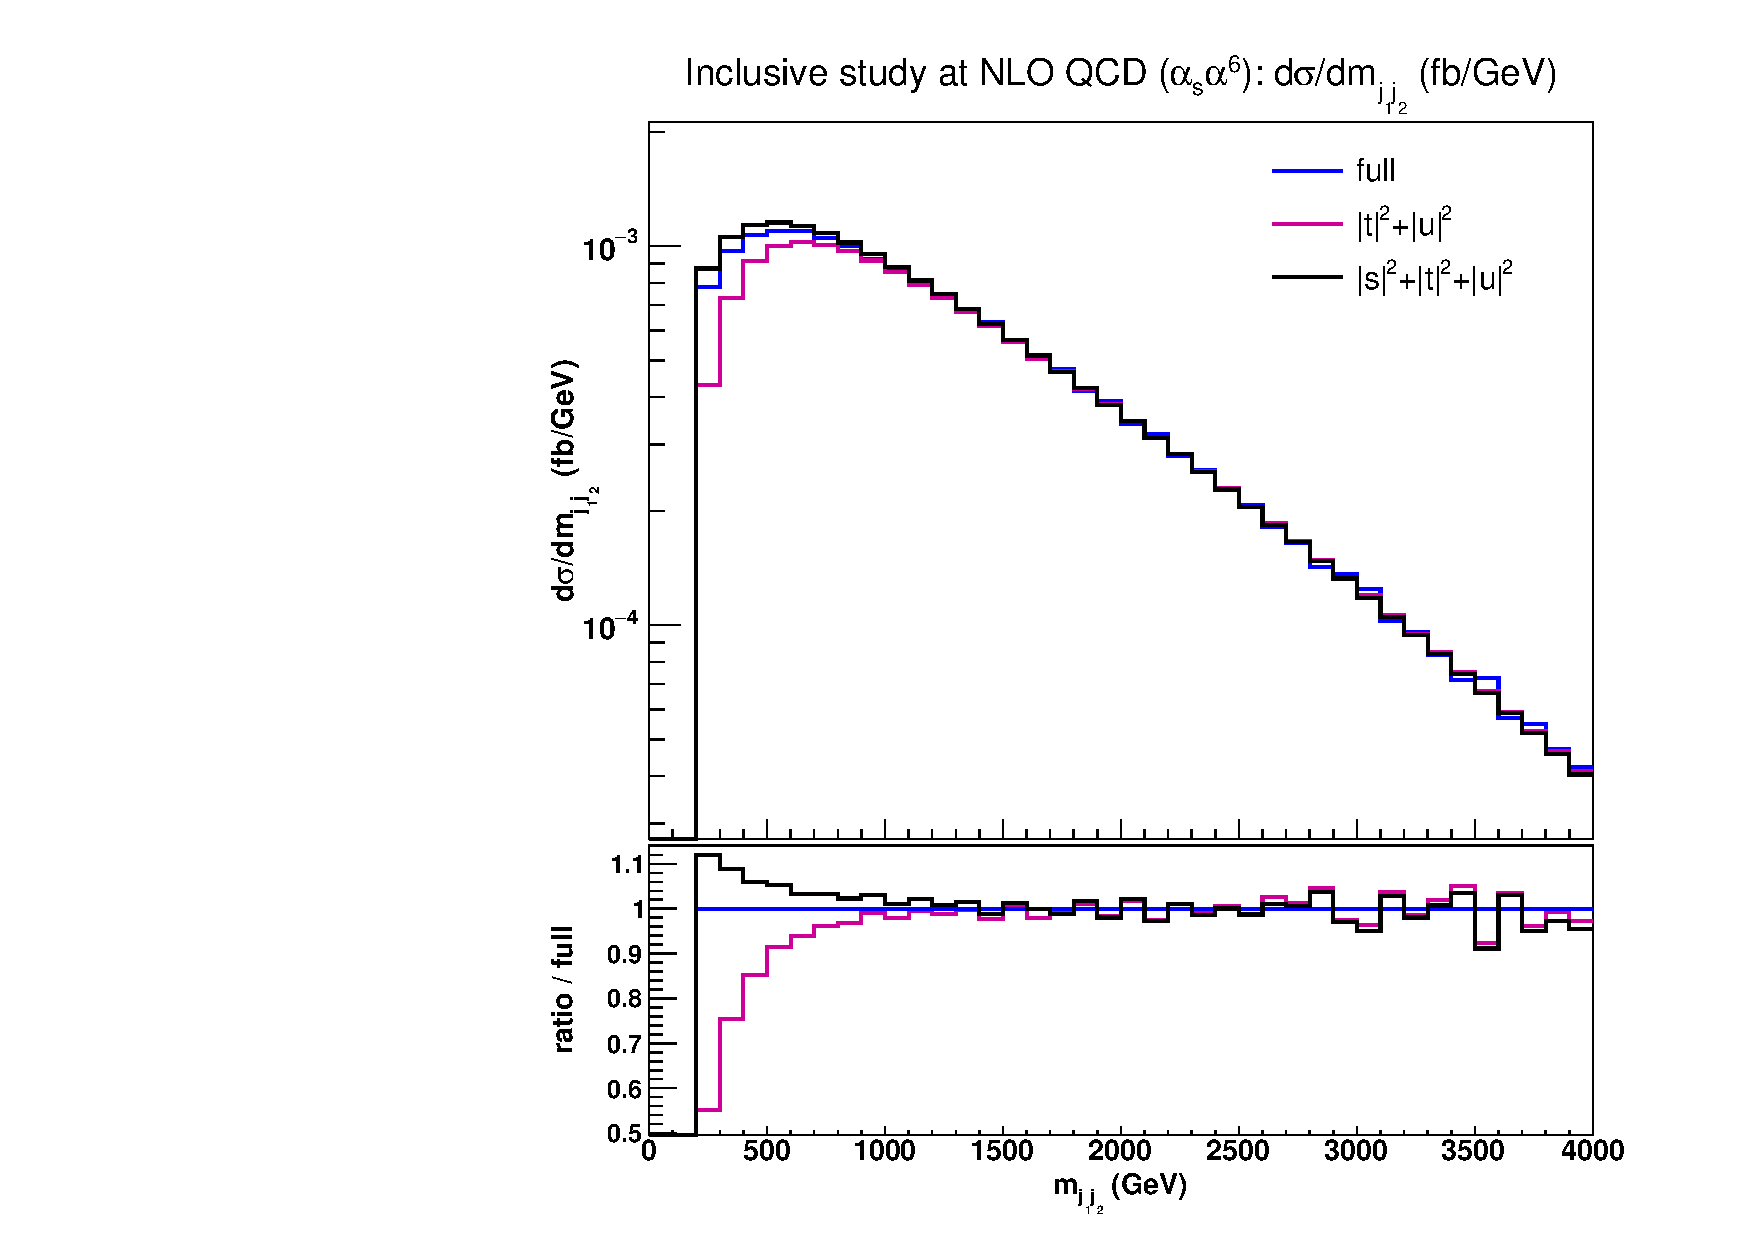
\includegraphics[scale=0.35]{figures/scanfigures/mjj_nlo.pdf}}
{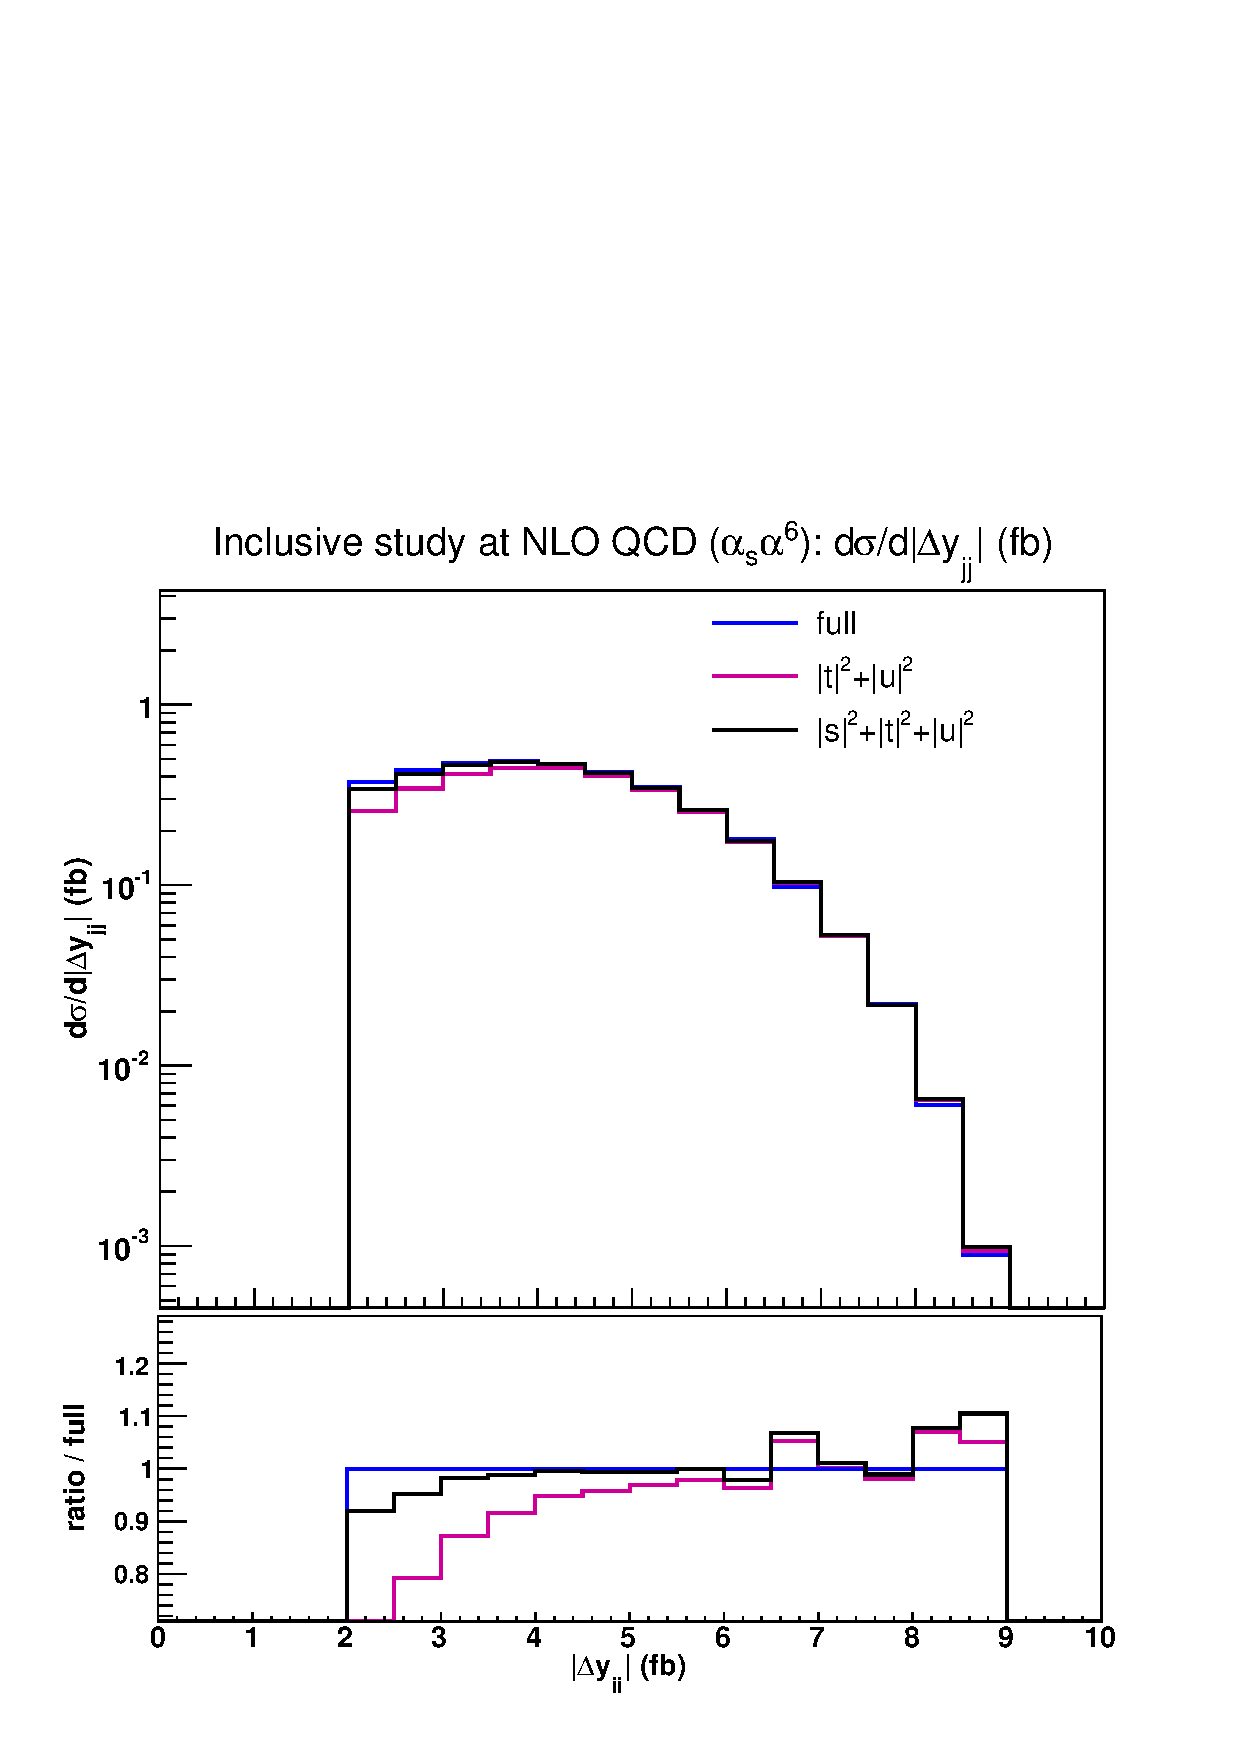
\includegraphics[scale=0.35]{figures/scanfigures/dyjj_nlo.pdf}}
\caption{NLO QCD inclusive study: distributions in $m_{\Pj\Pj}$ (left) and $\Delta y_{\Pj\Pj}$ (right), obtained with full ({\sc Recola}) and approximated ({\sc VBFNLO, Bonsay}) amplitudes at order $\mathcal{O}(\alphas\alpha^6)$.} \label{fig:mjjdyjj_1d_1}
\end{figure}


\begin{figure}[h]
\centering
{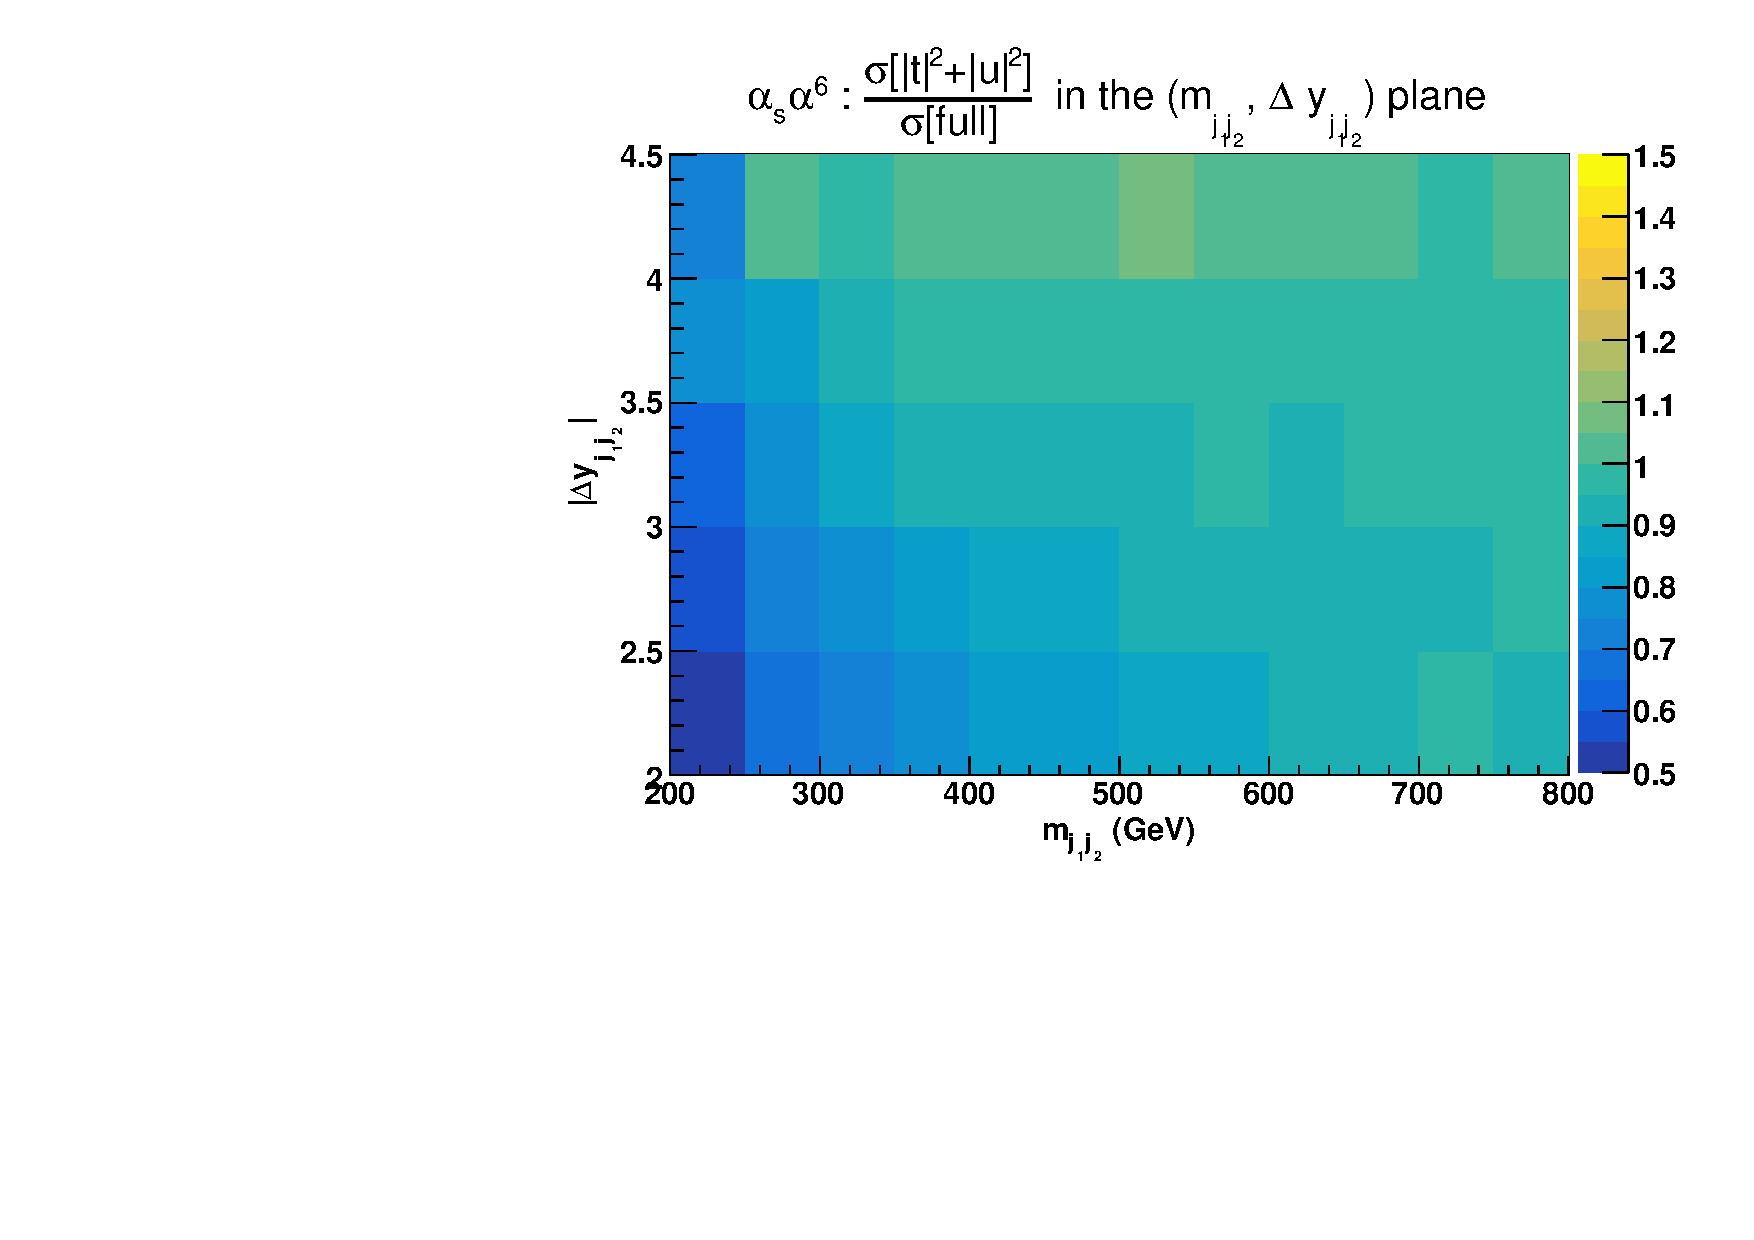
\includegraphics[scale=0.39]{figures/scanfigures/a6as_vbfnloVSrecola_tu.pdf}}
%\includegraphics[scale=0.395]{figures/scanfigures/.pdf}
\caption{Cross sections (fb) per bin of $(m_{\Pj\Pj},\,\Delta y_{\Pj\Pj})$ at NLO QCD $\mathcal{O}(\alphas\alpha^6)$, without any cut on the $jj$ pair kinematics: ratio of approximated squared amplitudes over the full matrix element. The approximated squared amplitudes are computed as $|\mathcal{A}|^2 \sim |t|^2 + |u|^2$. Results of {\sc Bonsay} (approximated) and {\sc Recola} (full) calculations. {\bf GP: notation to be changed, Mjj > mjj, alphas alpha} }\label{fig:ratio2d_NLO}
\end{figure}
\begin{figure}[hbt]
\centering
{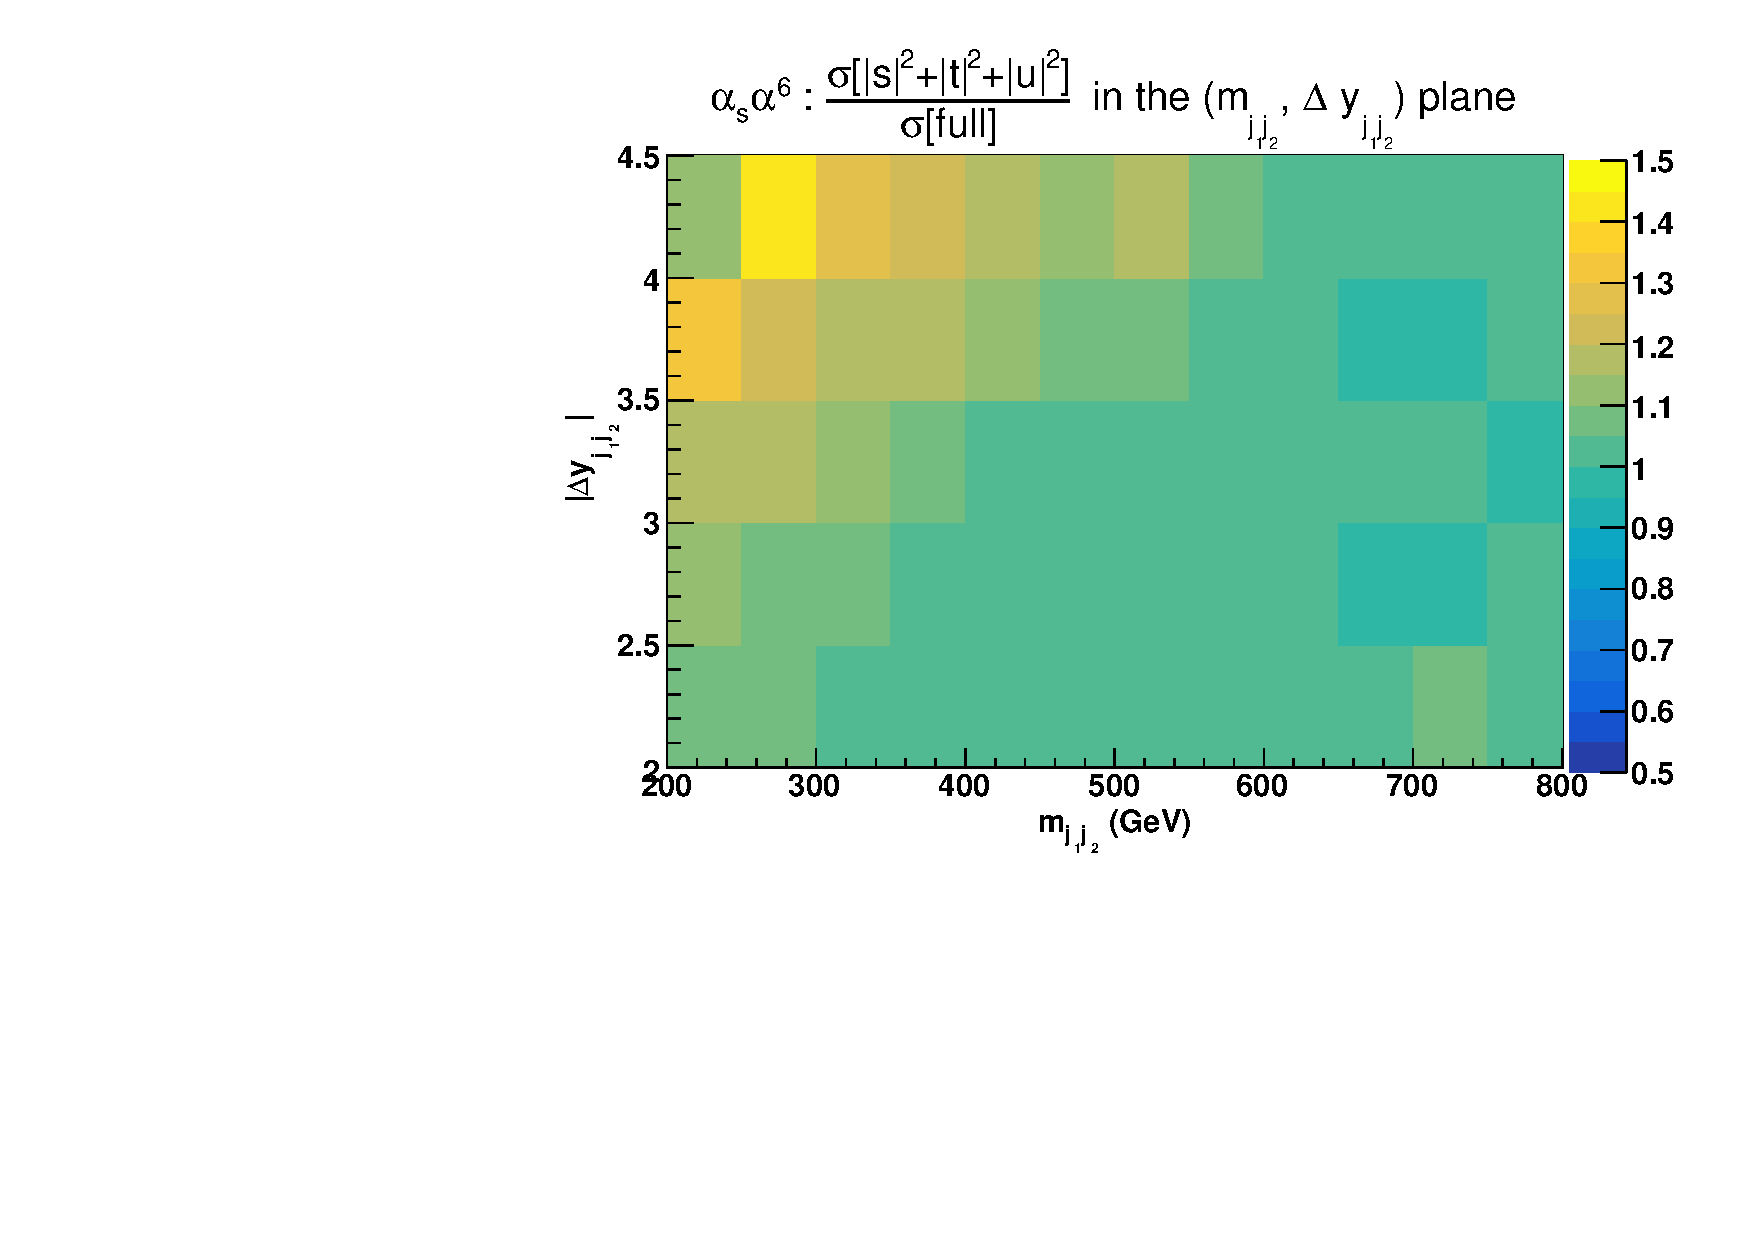
\includegraphics[scale=0.39]{figures/scanfigures/a6as_vbfnloVSrecola_stu.pdf}}
\caption{Cross section (fb) per bin of $(m_{\Pj\Pj},\,\Delta y_{\Pj\Pj})$ at NLO QCD $\mathcal{O}(\alphas\alpha^6)$, without any cut on the $jj$ pair kinematics:  ratio of approximated squared amplitudes over the full matrix element. The approximated squared amplitudes are computed as $|\mathcal{A}|^2 \sim |s|^2 + |t|^2 + |u|^2$. Results of {\sc VBFNLO} (approximated) and {\sc Recola} (full) calculations. {\bf GP: notation to be changed, Mjj > mjj, alphas alpha}}\label{fig:mjjdyjj_2d_NLO}
\end{figure}

As expected, in the low invariant mass--low rapidity separation region of the jet pair the VBS approximation fails badly (up to $40\%$ discrepancies).
The inclusion of the $s$-channel brings down to at most $5\%$.
However, the positive discrepancy shown in the low $m_{\Pj\Pj}$ region (black curve on Fig.~\ref{fig:mjjdyjj_1d_1}) can be traced back to the low $m_{\Pj\Pj}$, large $\Delta y_{\Pj\Pj}$ region of Fig.~\ref{fig:mjjdyjj_2d_NLO}.
In this region, the two leading jets have soft transverse momenta, according to the following low-angle approximation

\begin{equation}
\begin{split}
m_{\Pj_i\Pj_j}^2 &= 2\,\ptsub{\Pj_i}\ptsub{\Pj_j}\,(\cosh \Delta y_{\Pj_i\Pj_j} - \cos \Delta\phi_{\Pj_i\Pj_j}) \\
&\approx 2\,\ptsub{\Pj_i}\ptsub{\Pj_j}\,\cosh \Delta y_{\Pj_i\Pj_j} \,\,.
\end{split}
\end{equation}

The same positive discrepancy for the $|s|^2 + |t|^2 + |u|^2$ approximation, can be seen in the low $\pt$ region of the leading jet in the left panel of Fig.~\ref{fig:mjjdyjj_1d_2}.
In the large invariant mass--small rapidity separation region of Fig.~\ref{fig:mjjdyjj_2d_NLO}, discrepancies at the level of $15\%$ are present.
This can be traced back to the large $\pt$ and central rapidity region of the leading jets kinematics, shown in Fig.~\ref{fig:mjjdyjj_1d_2}. For such distributions, despite the $s$-channel inclusion, the discrepancy between the approximated and full result is about 5-10 \%.\\
In the VBS signal-region the VBS approximation shows a good agreement with the full calculation as documented in details below.

\begin{figure}[hbt]
\centering
{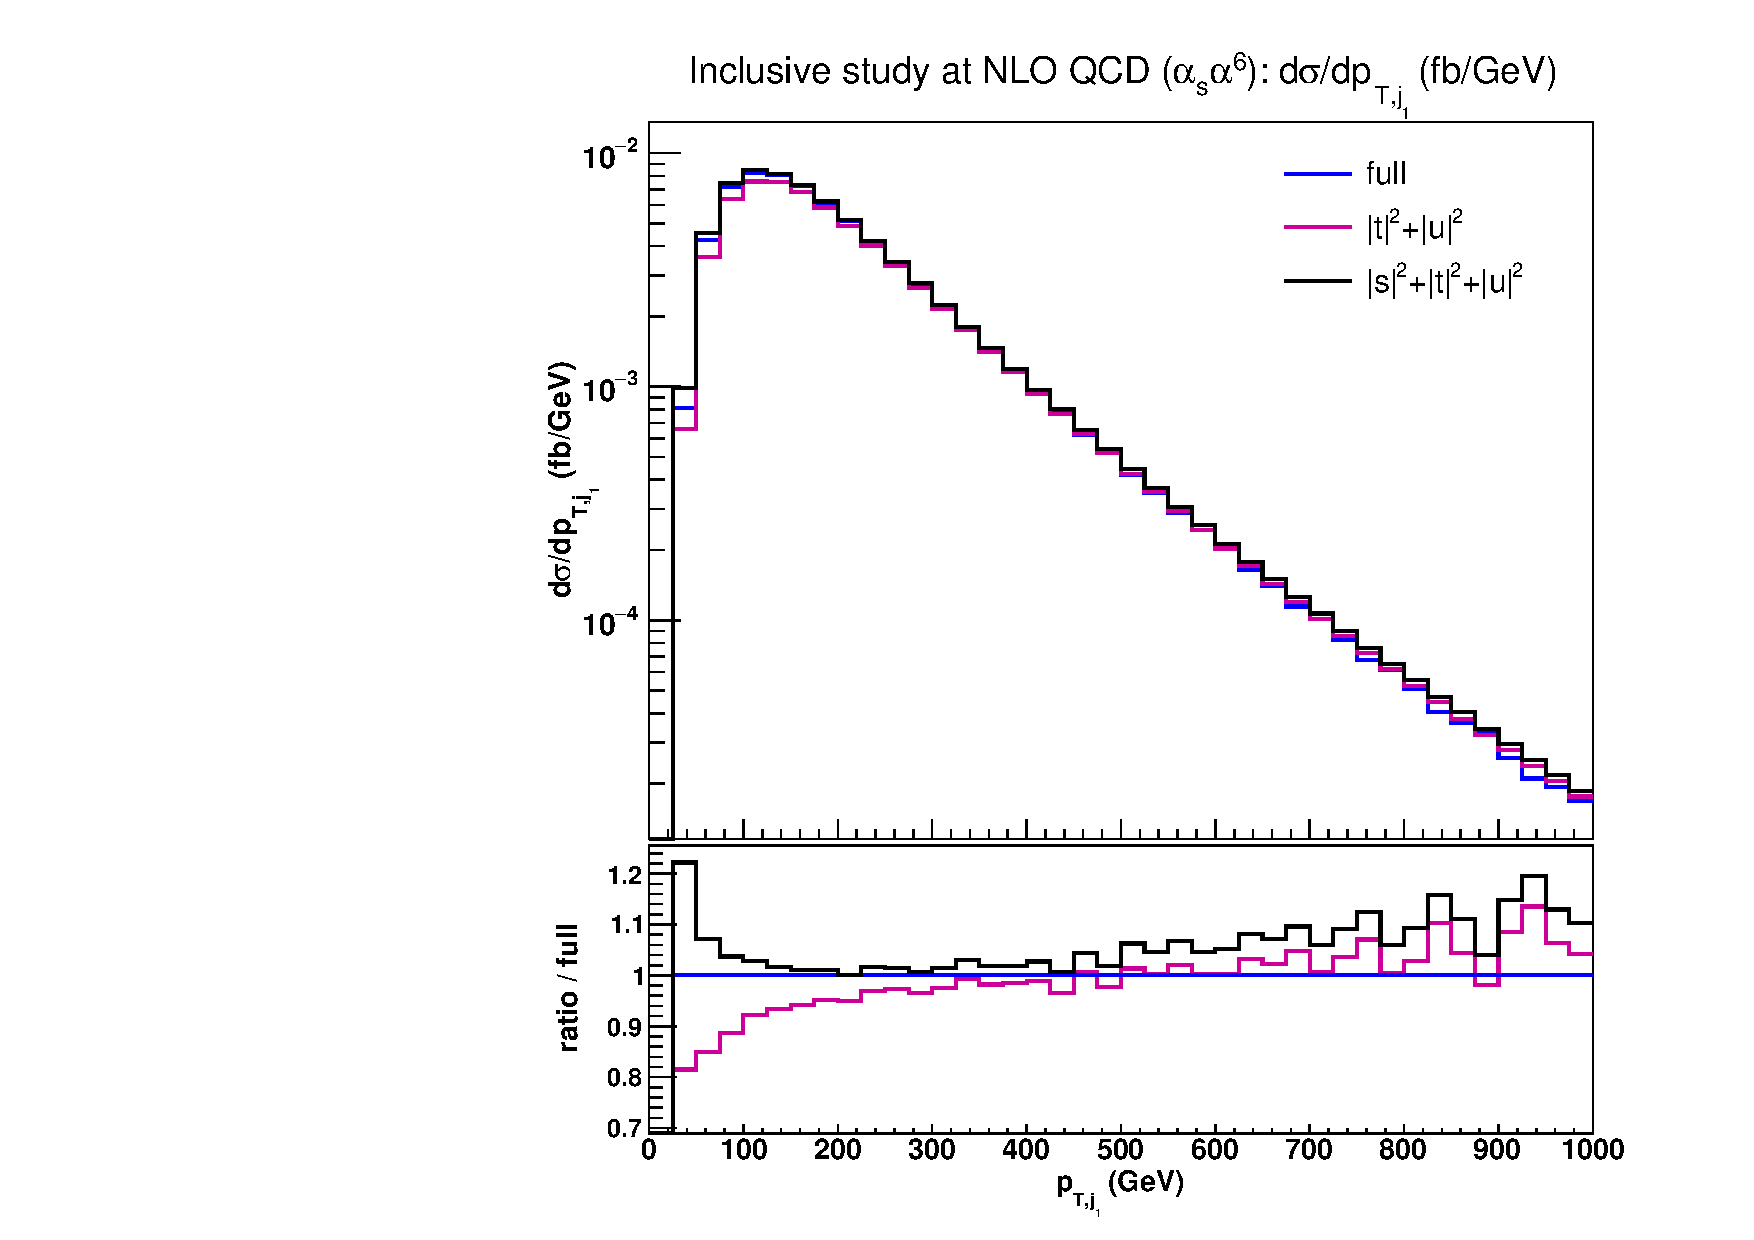
\includegraphics[scale=0.35]{figures/scanfigures/ptj1_nlo.pdf}}
{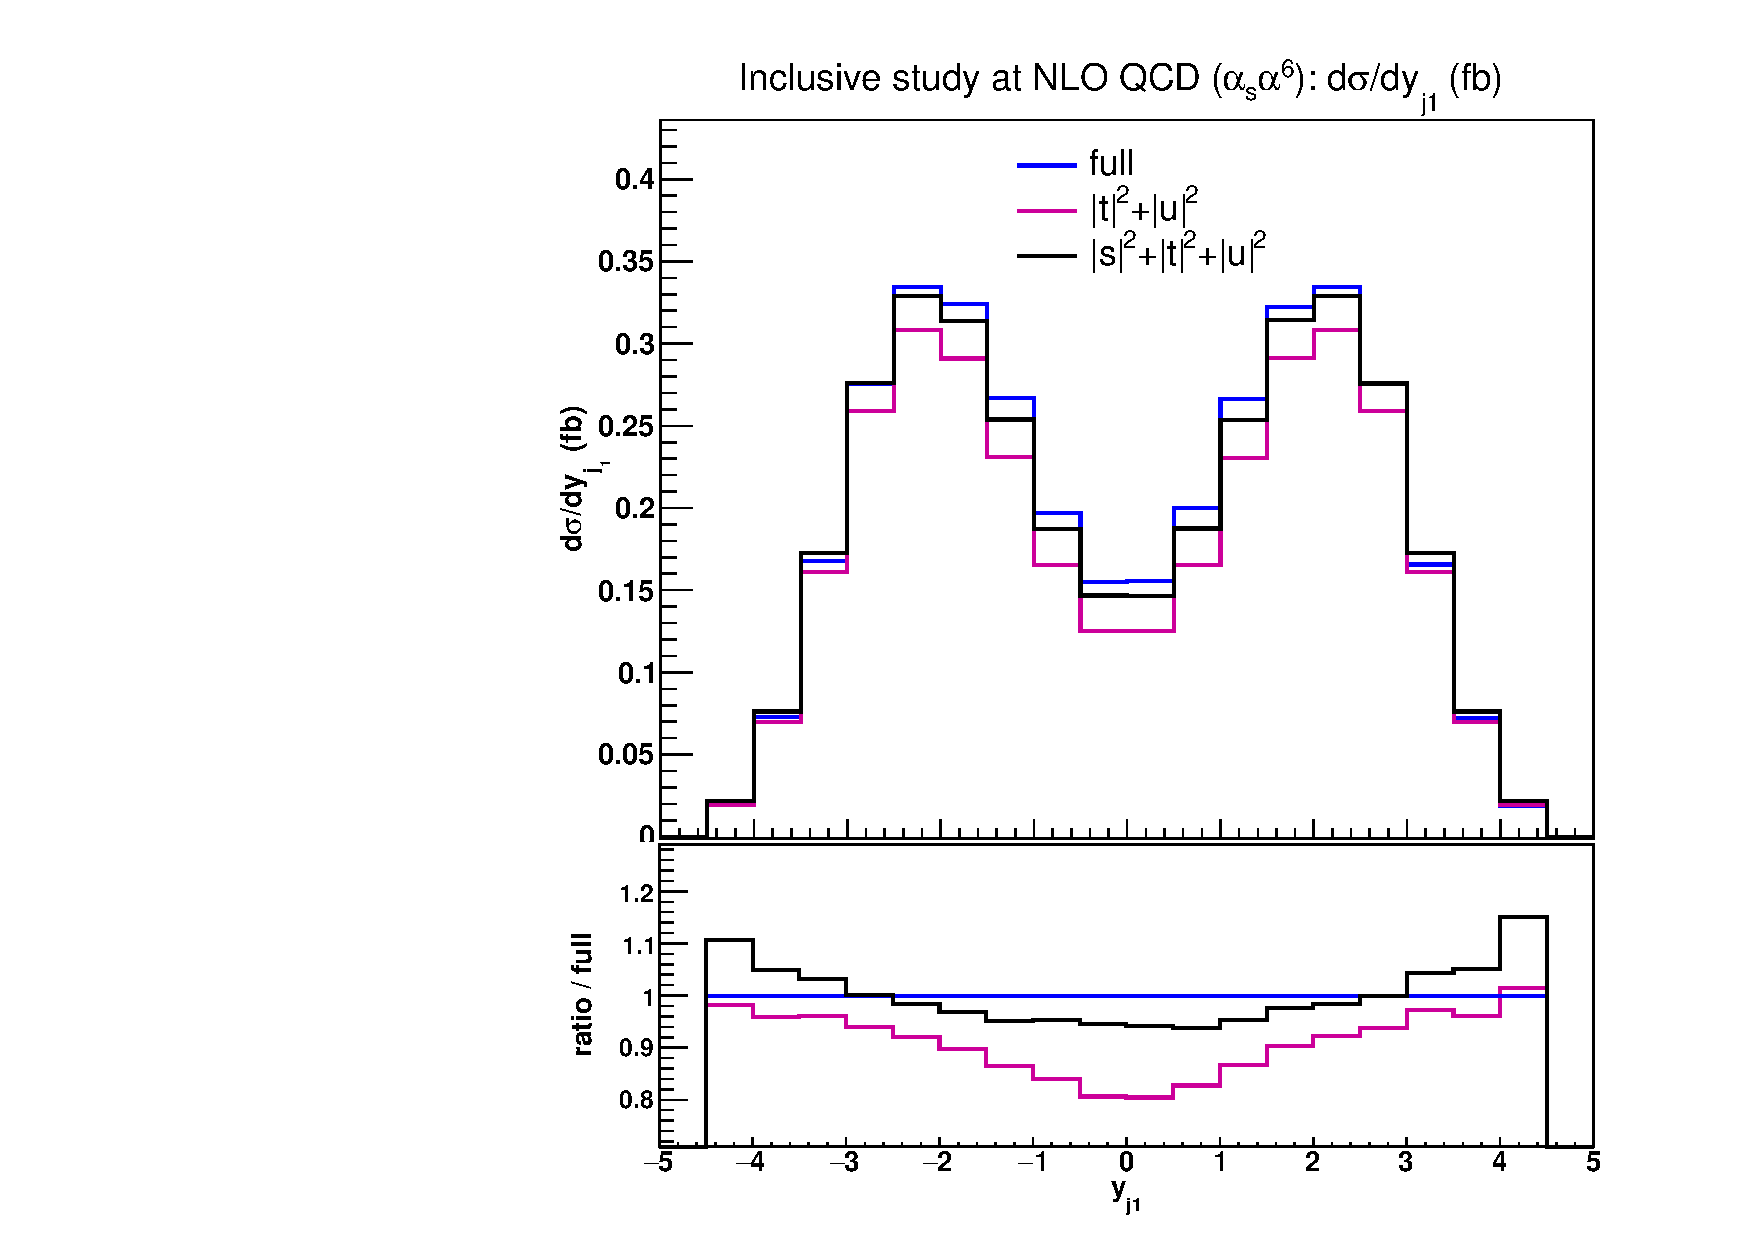
\includegraphics[scale=0.35]{figures/scanfigures/yj1_nlo.pdf}}
\caption{NLO QCD inclusive study: transverse momentum and rapidity distributions of the leading jet, obtained with full ({\sc Recola}) and approximated ({\sc VBFNLO, Bonsay}) amplitudes at order $\mathcal{O}(\alphas\alpha^6)$.} \label{fig:mjjdyjj_1d_2}
\end{figure}

Concerning leptonic kinematics, we show in Fig.~\ref{fig:mjjdyjj_1d_3} the distributions of the lepton-lepton invariant mass and of the Zeppenfeld variable of the electron \MP{We should defined the Zep var. somewhere}.

\begin{figure}[hbt]
\centering
{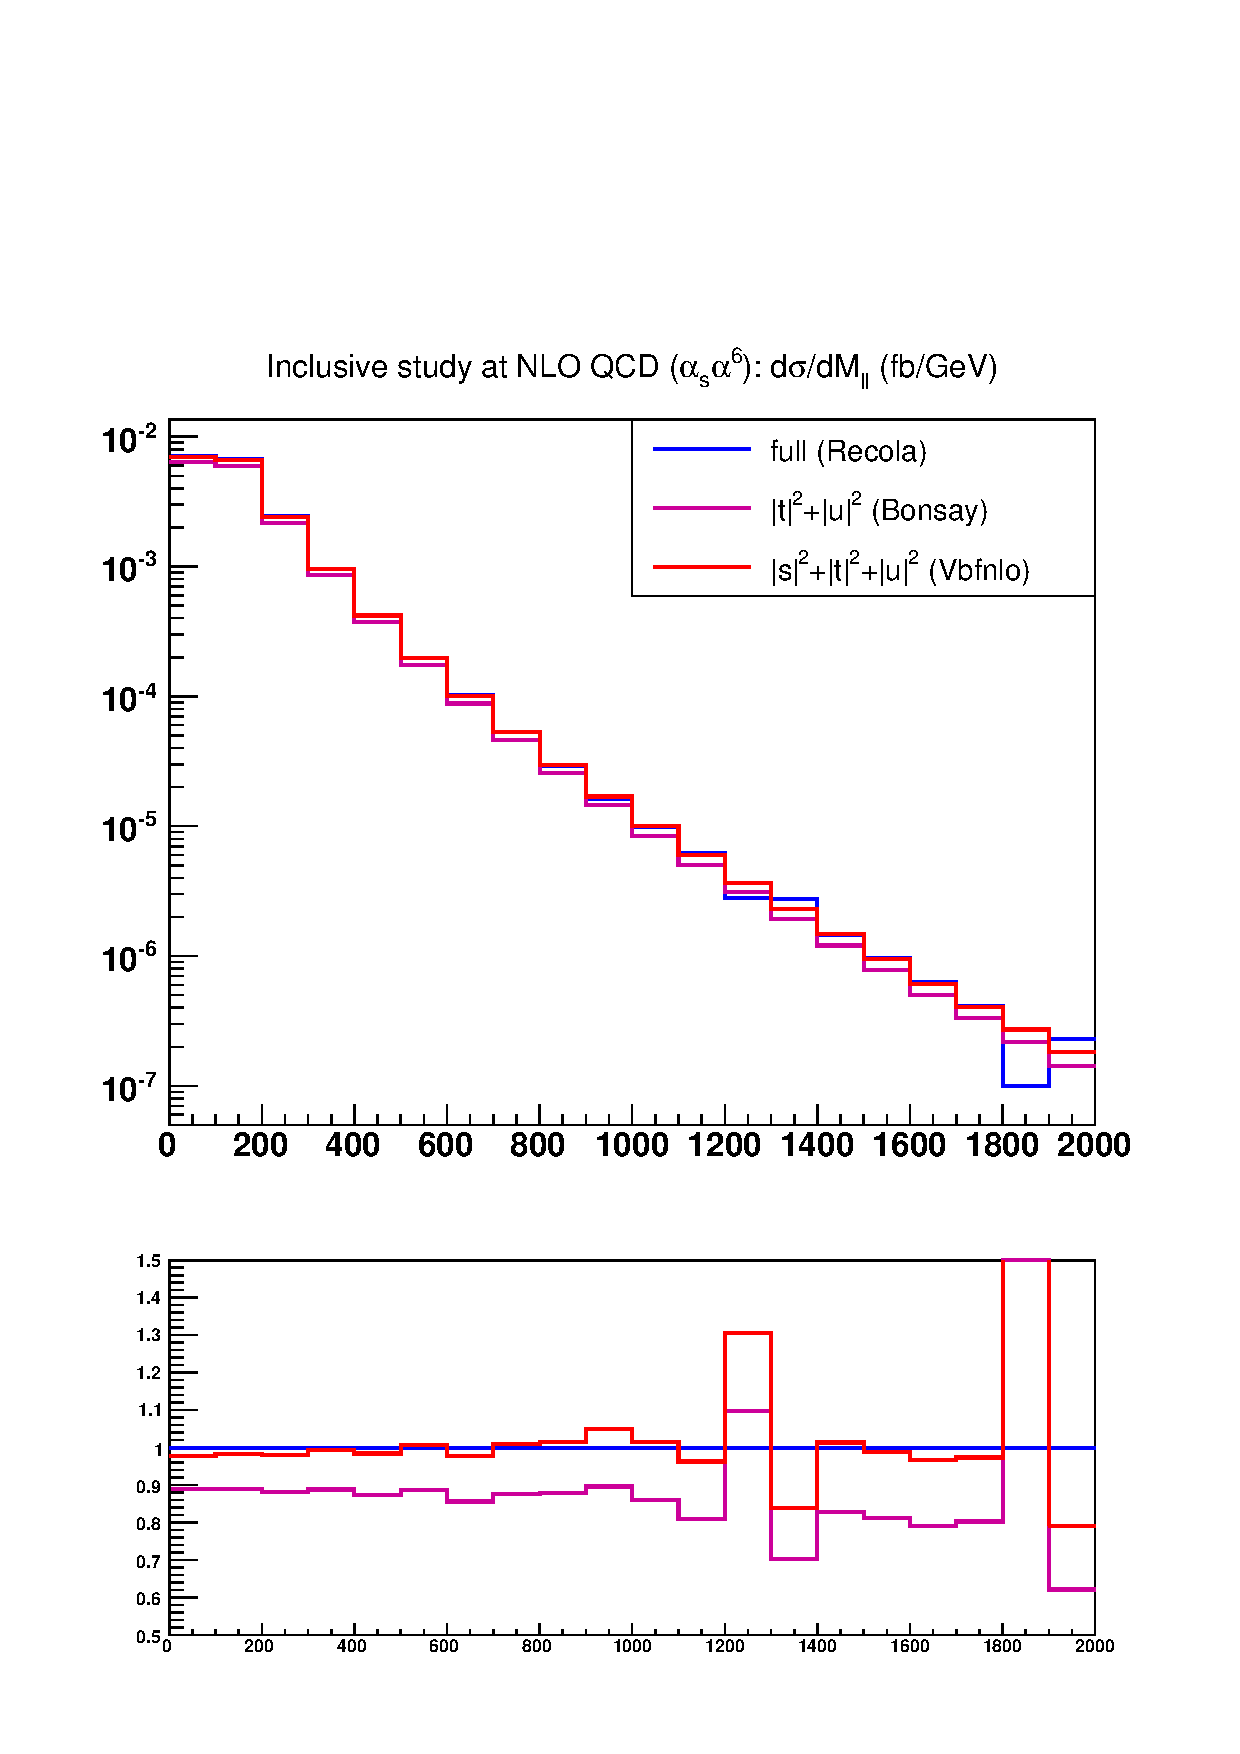
\includegraphics[scale=0.35]{figures/scanfigures/mll_nlo.pdf}}
{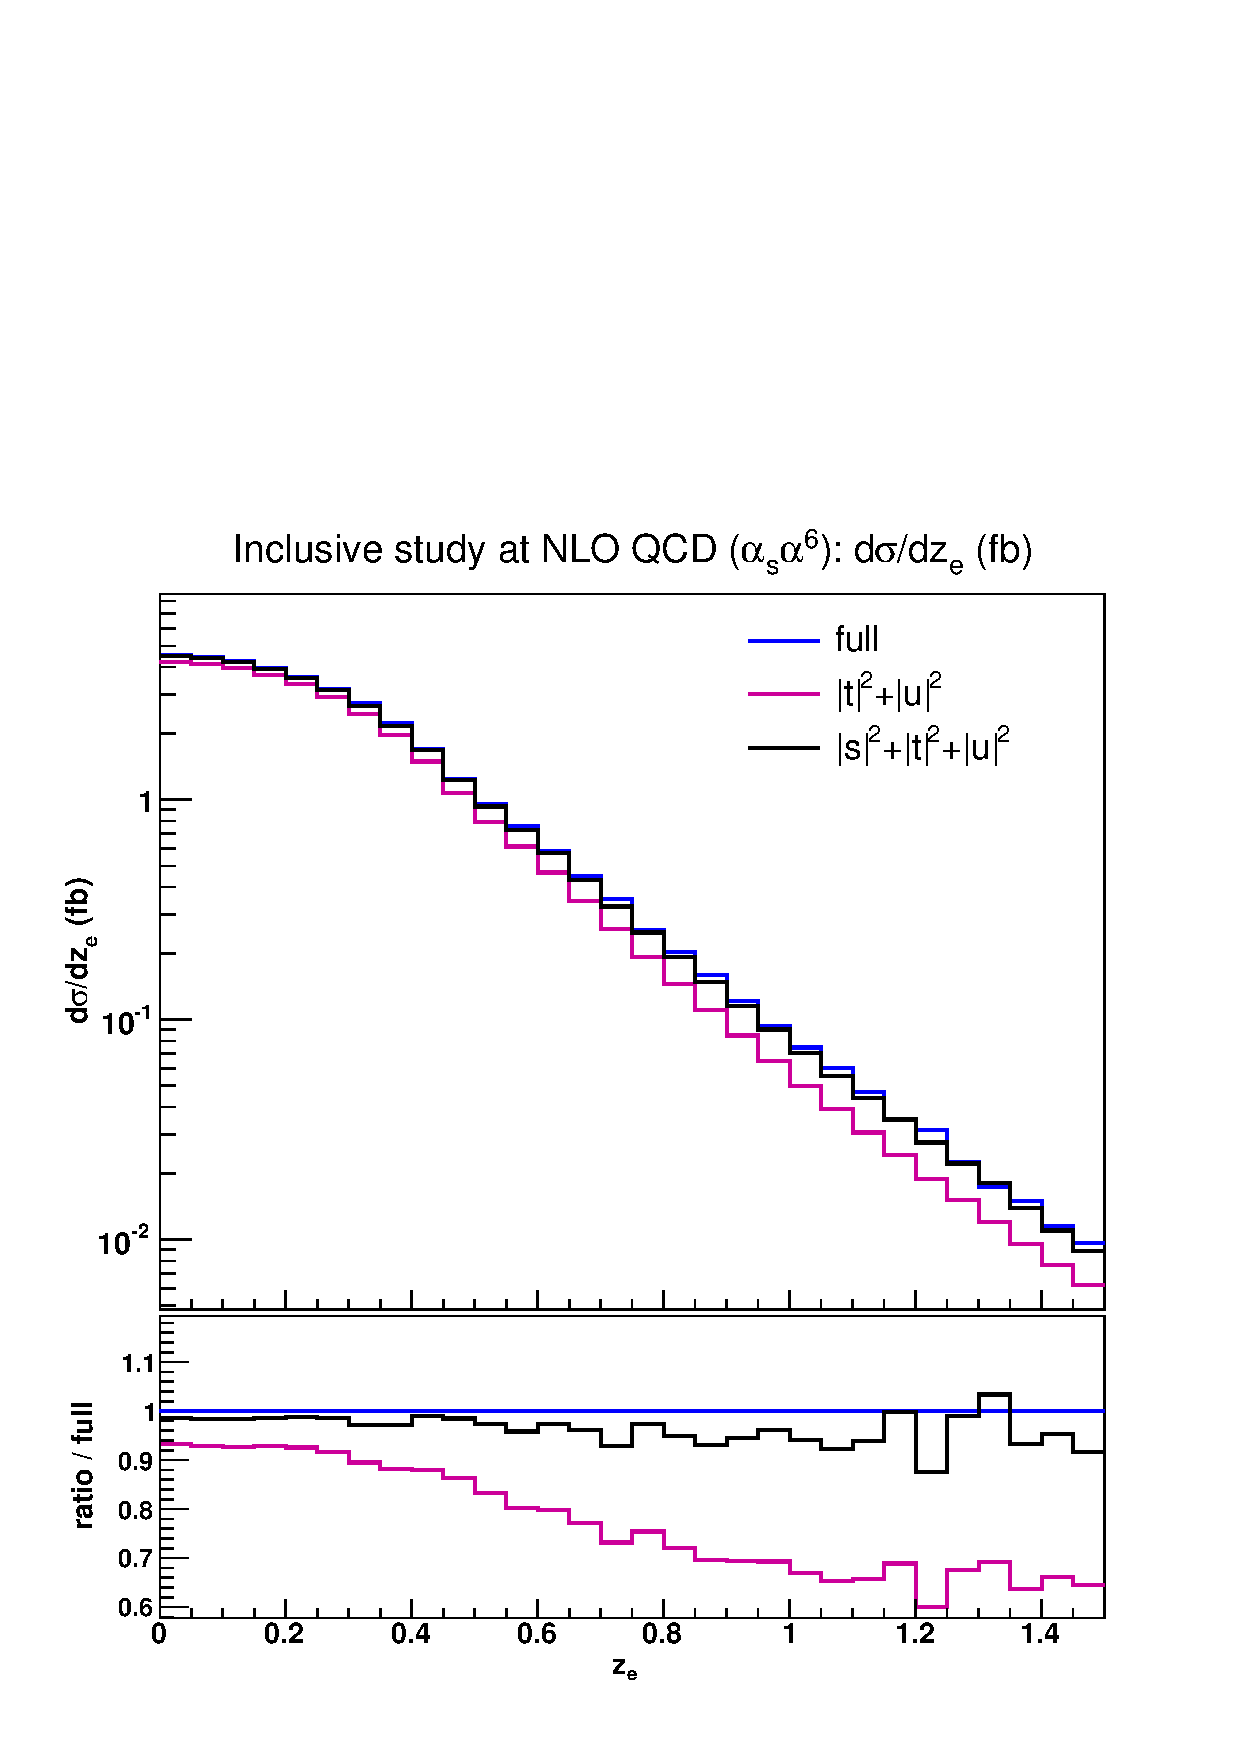
\includegraphics[scale=0.35]{figures/scanfigures/zel_nlo.pdf}}
\caption{NLO QCD inclusive study: distributions of the lepton--lepton invariant mass and the electron Zeppenfeld variable, obtained with full ({\sc Recola}) and approximated ({\sc VBFNLO, Bonsay}) amplitudes at order $\mathcal{O}(\alphas\alpha^6)$.} \label{fig:mjjdyjj_1d_3}
\end{figure}
{\bf GP: leptonic variables, comment further.}


In conclusion, both the loose minimum di-jet invariant mass cut and the inclusion of QCD radiative correction make the $s$-channel contributions less suppressed than at LO, making their inclusion mandatory, in order to provide trustworthy predictions at NLO accuracy.
Nevertheless, interferences and non-factorizable QCD corrections should be included to reduce the discrepancies down to the $\approx 1\%$  level, mainly in inclusive analyses.
Instead, the VBS approximation at NLO provides a good approximation of full calculations in the kinematic region where VBS contributions are dominant ($M_{\Pj\Pj} \gtrsim 600 \GeV$, $\Delta y_{\Pj\Pj} \gtrsim 3$), for both total cross section and differential distributions.
